\documentclass[pstricks,mathserif]{beamer}
\usetheme{Hannover}
\usefonttheme[onlymath]{serif}


\usepackage{graphicx}
%\usepackage[T1]{fontenc}
\usepackage[utf8]{inputenc}
\usepackage{amsmath, amssymb,amsthm}
\usepackage{comment}
%\usepackage{url} 
\usepackage{bm}
%\usepackage{esint}
\usepackage{multirow}
%\usepackage{thmtools, thm-restate}
\usepackage{mathtools}
%\usepackage{framed}
%\usepackage{float}
%\usepackage{subcaption}
\usepackage{epstopdf}%New addition
%\usepackage{cite}
%\usepackage{subcaption}
\usepackage{subfig}
\usepackage[percent]{overpic}
\usepackage[absolute,overlay]{textpos}


\definecolor{firstcolor}{HTML}{F5F5FF}
\definecolor{secondcolor}{HTML}{EBEBFF}
\definecolor{thirdcolor}{HTML}{E0E0FF}
% Recreate the commands for equations
%\renewcommand*{\equationautorefname}{equation}
%\def\equationautorefname~#1\null{%equation~(#1)\null

%Trying to get a pyramid
  
\usepackage{tikz}
\usetikzlibrary{intersections}  
%\usetikzlibrary{hobby}
%\usepackage{multido}
%\SpecialCoor  
%\def\Pyramid#1{%
%    \begin{pspicture}(#1,-#1)
%    \multido{\i=1+1}{#1}{%
%        \pstriangle(!#1 2 div \i\space neg)(\i,\i)
%        \uput[90](!#1 2 div \i\space neg){\char\numexpr\i+64}}
%    \end{pspicture}}

%Commands

\newcommand\irregularcircle[2]{% radius, irregularity
  \pgfextra {\pgfmathsetmacro\len{(#1)+rand*(#2)}}
  +(0:\len pt)
  \foreach \a in {10,20,...,350}{
    \pgfextra {\pgfmathsetmacro\len{(#1)+rand*(#2)}}
    -- +(\a:\len pt)
  } -- cycle
}

\newcommand{\party}[2]{\frac{\partial{#1}}{\partial{#2}}}

\title{Jet evolution in a dense QCD medium}
\author{Linnéa Gräns Samuelsson}
\institute % (optional)
{
  Internship at CEA Saclay\\
  Supervisors: Edmond Iancu and Gregory Soyez
}
\begin{document}


\frame{\titlepage}


%\section{Structure}
\section{Intro}

\begin{frame}


\minipage{0.3\textwidth}
\endminipage\hfill
\minipage{0.7\textwidth}
\begin{itemize}
\item \emph{the medium: a quark gluon plasma created in a heavy ion collision}
\item \emph{the jet: a collimated spray of particles generated via successive branchings of a parton with high energy produced in the collision}
\end{itemize}
\endminipage\hfill


\vspace*{1cm}


Structure of presentation:

\begin{itemize}
\item Context
\item Physics
\item Stochastics
\item Numerics
\end{itemize}

\vspace*{1cm}

\end{frame}

\section{Context}

\begin{frame}

%\frametitle{\small \flushleft HIC's, QGP's and jets}
Heavy ion collisions, quark gluon plasma and jets,\\
what we observe:

\begin{center}
\includegraphics[width=1\linewidth]{CMS_JetQ.png}
\end{center}
%Note: this picture is misleading.
%This is one of the findings, fluctuations
%are large enough to compete with jets
%travelling a different distance through the medium

Di-jet asymmetry. Missing energy found among soft hadrons propagating at large angles $\Rightarrow$ different from in vacuum jet evolution.


\end{frame}



\begin{frame}
 %\begin{textblock}{0.5}(0.001,0.001)
 % Test
 %\end{textblock}
\vspace*{0.5cm}
Heavy ion collisions, quark gluon plasma and jets,\\
the stereotypical picture:
\begin{center}
\includegraphics[width=0.45\linewidth]{jet-quenching.jpg}
\end{center}
%Note: this picture is misleading.
%This is one of the findings, fluctuations
%are large enough to compete with jets
%travelling a different distance through the medium


Implicit assumption: small energy fluctuations.

\vspace*{0.5cm}

\minipage{0.5\textwidth}
	\centering
	\includegraphics[width=0.45\linewidth]{Dijet_flucts1.pdf}
\endminipage\hfill
\minipage{0.5\textwidth}
	\centering
  	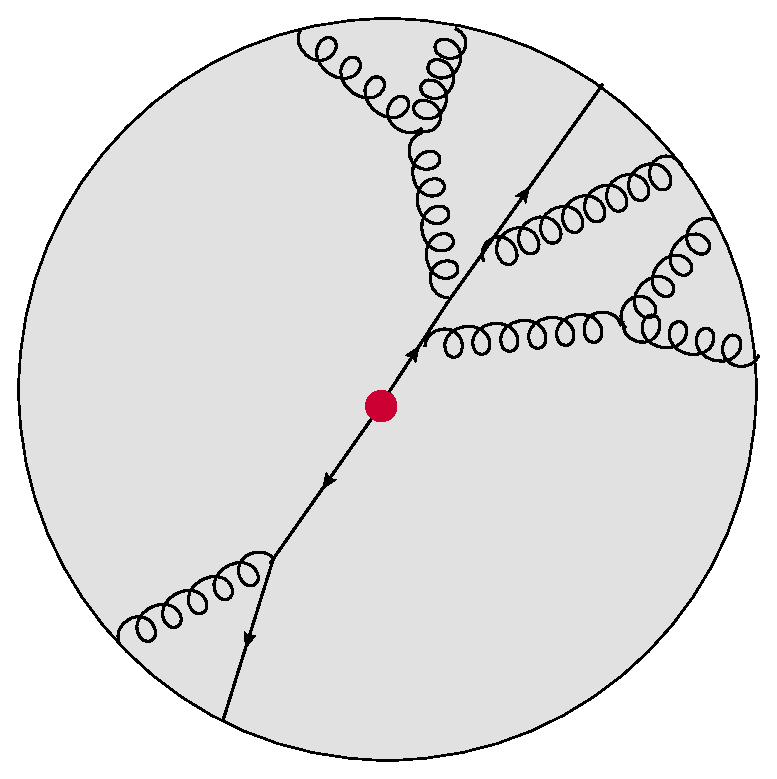
\includegraphics[width=0.45\linewidth]{Dijet_flucts2.eps}
\endminipage\hfill
\vspace*{1cm}

\end{frame}



\begin{frame}
We need a model that answers:
\begin{itemize}
\item How can the lost energy end up at such large angles?
\item How large are the energy fluctuations?
\end{itemize}
\end{frame}

\section{Physical picture}

\begin{frame}
\frametitle{Physical picture}

{\em In medium} scattering triggers emissions:
\begin{itemize}
\item Destroys quantum coherence
\item Gives broadening of transverse momentum
\end{itemize}


Formation time: $\lambda_\perp<\Delta x_\perp \Rightarrow \frac{1}{k_\perp}<\frac{k_\perp}{\omega}\Delta t_f .$

\begin{center}


\begin{tikzpicture}
    \node[anchor=south west,inner sep=0] (image) at (0,0) {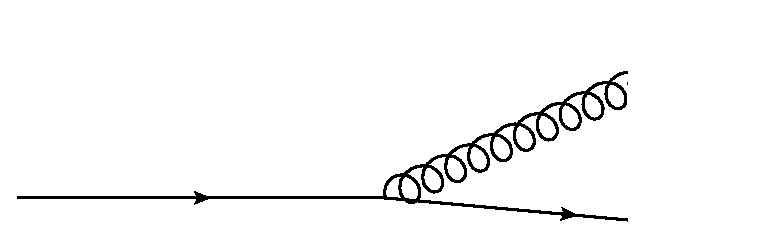
\includegraphics[width=0.5\textwidth]{gluonemission.eps}};
    \begin{scope}[x={(image.south east)},y={(image.north west)}]
        \draw[] (0.70,0.11) arc (-12:21:0.7);
        \node[] at (0.65, 0.7) {$\omega,k_\perp$};
        \node[] at (0.74, 0.27) {$\theta$};
        \draw[red,thick,dashed, <->] (0.83,0.1) -- (0.83,0.7);
        \node[red,right] at (0.83, 0.35){$\Delta x_\perp$};
        \draw[blue,thick, dashed,<->] (0.5,0) -- (0.83,00);
        \node[blue,below] at (0.65, 0){$\Delta t_f$};
    \end{scope}
\end{tikzpicture}
\end{center}
\end{frame}
\begin{frame}



$\Delta t_f \gg $ mean free path $\gg$ Debye length $\Rightarrow$  multiple scatterings lead to one emission and scattering centers are independent  $\Rightarrow$ random walk $\Rightarrow$ $\langle k_\perp^2 \rangle \sim \hat{q}\Delta t$.

\begin{center}
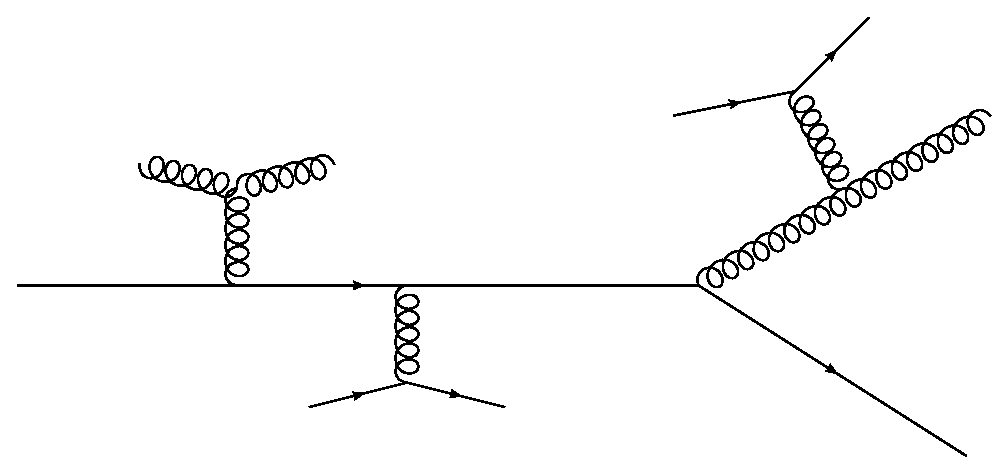
\includegraphics[width=0.5\linewidth]{scattering.eps}
\end{center}



All together: $\Delta t_f \sim \sqrt{\frac{\omega}{\hat{q}}}$ 
and $\theta_f=\left( \frac{\hat{q}}{\omega^3} \right)^{1/4}$

$\Rightarrow$ we favour soft gluons at large angles!

\end{frame}

\begin{frame}

If instead $\omega$ energy of parent: $\Delta P (z, \omega, \Delta t) \sim \alpha_s \Delta t/ [\Delta t_f(z\omega)]$
\vspace*{-0.5cm}
\begin{itemize}
\item For $z \omega \sim \omega_{br}$,
$\Delta P (z, \omega) \sim \mathcal{O}(1)$ at $\Delta t = L$  
\item For $\omega_{br}$, $P(z, \omega_{br}) \sim \mathcal{O}(1)$ for $\Delta t < L$, even for $z \sim 1-z$
\end{itemize}
\vspace*{0.7cm}
$\Delta P\sim \mathcal{O}(1)$\\
$\Rightarrow$ multiple branching!\\
A typical event:
\vspace*{-2cm}
\begin{center}
\begin{overpic}[width=0.6\linewidth]{democraticbranch.eps}
	\put(5,45){$E$}
	\put(59,49){$\omega \sim \omega_{br}$}
	\put(86,36){{\color{gray}$\omega \ll \omega_{br}$}}
	\put(46,76){$(1-z) \omega$}	
	\put(71,59){$z \omega$}
	\put(100,58){$T$}
	\put(96,76){$T$}
\end{overpic}
\end{center}
\vspace*{-0.5cm}
%
\begin{itemize}
\small
\item A number of $\mathcal{O}(1)$ of primary gluons with $\omega \sim \omega_{br}$ emitted from leading particle.
\item They then branch democratically, transferring away all energy.
\item Hence both energy loss and its fluctuations on the scale $\omega_{br}$.
\end{itemize}
%
%
\end{frame}


\section{Markov process}



\begin{frame}
\frametitle{Markov process}
In medium evolution as a Markovian process. Branching rate from BDMPSZ spectrum:
$$\frac{\mathrm{d}^2 P(z,\tau)}{\mathrm{d}z\mathrm{d}\tau}=\frac{K(z)}{2 \sqrt{x}} \equiv K(x,z).$$


Splitting kernel: $K(z)=\frac{[1-z(1-z)]^{5/2}}{[z(1-z)]^{3/2}}$. 

Simplified: $K(z)=\frac{1}{[z(1-z)]^{3/2}}$.\\
~\\


Get equation for the one point function
$D(x,\tau)\equiv xn(x,\tau)$ 

\begin{center}
\includegraphics[width=0.9\linewidth]{RateEq_D.pdf}
\end{center}


and similarly (but longer) for the two-point function $D^{(2)}(x,x'\tau)\equiv xx'n^{(2)}(x,x',\tau)$.
%\includegraphics[width=0.8\linewidth]{RateEq_D2.pdf}

%$\party{}{\tau}D(x,\tau)=\int \mathrm{d}z\, K(z) \left[\sqrt{\frac{z}{x}} D\left(\frac{x}{z},\tau\right)- \frac{z}{\sqrt{x}}D(x,\tau)  \right]$
\end{frame}


\begin{frame}
Simple kernel:
\includegraphics[width=0.9\linewidth]{plotD.pdf}

\begin{itemize}
\item Energy fraction left in gluon cascade: $\int_0^1 \mathrm{d}x\, D(x,\tau) = e^{-\pi\tau^2}$ $\Rightarrow$ decreasing in time. 
\item Formally: condensate at $x=0$. Physically: thermalization.
\item At small $\tau$, loss $\simeq \pi \omega_{br}$. 
\item $D^{(2)}(x,x'\tau)$ used to find fluctuations. To order $\tau^4$:
 $$\sigma_\epsilon(\tau)\simeq \langle \epsilon(\tau)\rangle/\sqrt{3}$$.
\end{itemize}
 

%\vspace*{1cm}
%Note: (fix point...)
%Democratic branching compared to wave turbulence. Might actually end up skipping this part.\\
%~\\

%{\tiny
%\minipage{0.5\textwidth}
%	\centering
%	\begin{overpic}[width=0.7\linewidth]{democratic.eps}
	%\put(5,40){$x=1$}
	%\put(43,47){$x \sim \frac{1}{2}$}
	%\put(53,58){$x \sim \frac{1}{4}$}
	%\put(68,59){\vector(4,0){8}}
	%\put(64,70){$x \sim \frac{1}{8}$}
	%\put(79,71){\vector(4,0){8}}
%	\end{overpic}
  	%\vspace*{-30pt}
  	%\caption{here go gluons}\label{fig:D0_t1}
%\endminipage\hfill
%\minipage{0.5\textwidth}
%	\centering
%  	\includegraphics[width=0.7\linewidth]{Richardson_cascade.png}
  	%\vspace*{-30pt}
  	%\caption{Turbulence}\label{fig:D0_t5}
%\endminipage\hfill
%}


\end{frame}



\section{Monte Carlo simulation}

\begin{frame}
\frametitle{Monte Carlo simulation}

Result: full kernel $\Rightarrow$ less efficient branching\\
~\\

%\vspace*{1cm}


\minipage{0.5\textwidth}
\centering
\small $\sqrt{x} D(x)$
\includegraphics[width=1\linewidth]{times.pdf}
\endminipage\hfill
\minipage{0.5\textwidth}
%\centering
\small 

Simple splitting kernel, numerical versus analytic:
\begin{itemize}
\item Good agreement overall
\item Bias at small x (pileup)
\end{itemize}

Corrections from the full splitting kernel:
\begin{itemize}
\item Leading peak still present at $\tau=0.5$
\item Less energy lost at $\tau=1$
\end{itemize}


Recall:

Simple $K(z)=\frac{1}{[z(1-z)]^{3/2}}$


Full $K(z)=\frac{[1-z(1-z)]^{5/2}}{[z(1-z)]^{3/2}}$


\endminipage\hfill


\end{frame}


\begin{frame}
\frametitle{Monte Carlo simulation}

Result: full kernel $\Rightarrow$ less efficient branching\\
~\\

%\vspace*{1cm}


\minipage{0.5\textwidth}
\centering
\small $\sqrt{x} D(x)$
\includegraphics[width=1\linewidth]{times.pdf}
\endminipage\hfill
\minipage{0.5\textwidth}
\centering
\small $x D^2(x,x)$
\includegraphics[width=1\linewidth]{D2.pdf}
\endminipage\hfill


\end{frame}



\begin{frame}
Energy loss: $1 - \int_0^1 \mathrm{d}x\, D(x,\tau) = 1 - e^{-\pi\tau^2}$
{\centering
\includegraphics[width=1\linewidth]{energyloss.pdf}
}
\end{frame}



\section{Outro}
\begin{frame}

%Maybe something about future work, discussion etc. I should probably have the thesis itself in a pdf viewer for easy reference in case of questions.

Summary:

\begin{itemize}
\item Democratic branchings $\Rightarrow$ energy found at large angles
\item Prediction: large fluctuations in energy loss
\item Possible to make Monte Carlo simulation
\item Full kernel $\Rightarrow$ less efficient branching
\item Full and simple kernel have same behaviour {\em qualitatively}
\end{itemize}
~\\
\center THE END\\
~\\
Questions?

\end{frame}

\end{document}